\documentclass[11pt]{article}

\usepackage{fix-cm}
\usepackage{tikz}
\usetikzlibrary{shapes,backgrounds,calc,patterns}
\usepackage{amsmath,amsthm} 
\usepackage{amssymb}
\usepackage[framemethod=tikz]{mdframed}
\usepackage{C:/Users/paulb/VSTeX/local/draculatheme}
\usepackage{mathrsfs}
\usepackage{changepage}
\usepackage{multicol}
\usepackage{mathtools}
\usepackage{hyperref}
\usepackage{slashed}
\usepackage{enumerate}
\usepackage{booktabs}
\usepackage{enumitem}
\usepackage{kantlipsum} 
\usepackage{pgfplots}
\pgfplotsset{compat=1.18}
\usetikzlibrary{decorations.markings}

\setlength{\parindent}{0pt}

\newmdenv[
  topline=false,
  bottomline=true,
  rightline=false,
  leftline=true,
  linewidth=1.5pt,
  linecolor=black, % default color, will be overridden in custom commands
  backgroundcolor=draculabg, % Needed for Dracula theme
  fontcolor=draculafg, % Needed for Dracula theme
  innertopmargin=0pt,
  innerbottommargin=5pt,
  innerrightmargin=10pt,
  innerleftmargin=10pt,
  leftmargin=0pt,
  rightmargin=0pt,
  skipabove=\topsep,
  skipbelow=\topsep,
]{customframedproof}

\newenvironment{proofpart}[2][black]{
    \begin{mdframed}[
        topline=false,
        bottomline=false,
        rightline=false,
        leftline=true,
        linewidth=1pt,
        linecolor=#1!40, % Custom color
        % innertopmargin=10pt,
        % innerbottommargin=10pt,
        innerleftmargin=10pt,
        innerrightmargin=10pt,
        leftmargin=0pt,
        rightmargin=0pt,
        % skipabove=\topsep,
        % skipbelow=\topsep%
    ]
    \noindent
    \begin{minipage}[t]{0.08\textwidth}%
        \textbf{#2}%
    \end{minipage}%
    \begin{minipage}[t]{0.90\textwidth}%
        \begin{adjustwidth}{0pt}{0pt}%
}{
    \end{adjustwidth}
    \end{minipage}
    \end{mdframed}
}

\newenvironment{solution}
  {\textit{Solution.}}



%%% AESTHETICS %%%
%-%-%-%-%-%-%-%-%-%-%-%-%-%-%-%-%-%-%-%-%-%-%-%-%-%-%-%-%-%-%-%-%-%-%-%-%-%-%


%%% Dimensions and Spacing %%%
\usepackage[left=0.5in,right=0.5in,top=1in,bottom=1in]{geometry}
% \usepackage{setspace}
% \linespread{1}
\usepackage{listings}

%%% Define new colors %%%
\usepackage{xcolor}
\definecolor{orangehdx}{rgb}{0.96, 0.51, 0.16}

% Normal colors
\definecolor{xred}{HTML}{BD4242}
\definecolor{xblue}{HTML}{4268BD}
\definecolor{xgreen}{HTML}{52B256}
\definecolor{xpurple}{HTML}{7F52B2}
\definecolor{xorange}{HTML}{FD9337}
\definecolor{xdotted}{HTML}{999999}
\definecolor{xgray}{HTML}{777777}
\definecolor{xcyan}{HTML}{80F5DC}
\definecolor{xpink}{HTML}{F690EA}
\definecolor{xgrayblue}{HTML}{49B095}
\definecolor{xgraycyan}{HTML}{5AA1B9}

% Dark colors
\colorlet{xdarkred}{red!85!black}
\colorlet{xdarkblue}{xblue!85!black}
\colorlet{xdarkgreen}{xgreen!85!black}
\colorlet{xdarkpurple}{xpurple!85!black}
\colorlet{xdarkorange}{xorange!85!black}
\definecolor{xdarkcyan}{HTML}{008B8B}
\colorlet{xdarkgray}{xgray!85!black}

% Very dark colors
\colorlet{xverydarkblue}{xblue!50!black}

% Document-specific colors
\colorlet{normaltextcolor}{black}
\colorlet{figtextcolor}{xblue}

% Enumerated colors
\colorlet{xcol0}{black}
\colorlet{xcol1}{xred}
\colorlet{xcol2}{xblue}
\colorlet{xcol3}{xgreen}
\colorlet{xcol4}{xpurple}
\colorlet{xcol5}{xorange}
\colorlet{xcol6}{xcyan}
\colorlet{xcol7}{xpink!75!black}

% Blue-Purple (should just used colorbrewer...)
\definecolor{xrainbow0}{HTML}{e41a1c}
\definecolor{xrainbow1}{HTML}{a24057}
\definecolor{xrainbow2}{HTML}{606692}
\definecolor{xrainbow3}{HTML}{3a85a8}
\definecolor{xrainbow4}{HTML}{42977e}
\definecolor{xrainbow5}{HTML}{4aaa54}
\definecolor{xrainbow6}{HTML}{629363}
\definecolor{xrainbow7}{HTML}{7e6e85}
\definecolor{xrainbow8}{HTML}{9c509b}
\definecolor{xrainbow9}{HTML}{c4625d}
\definecolor{xrainbow10}{HTML}{eb751f}
\definecolor{xrainbow11}{HTML}{ff9709}

%%% FIGURES %%%
\usepackage{graphicx}  
% \graphicspath{ {images/} }  
% \numberwithin{figure}{section}
\usepackage{float}
\usepackage{caption}

%%% Hyperlinks %%%
\usepackage{hyperref}
\definecolor{horange}{HTML}{f58026}
\hypersetup{
	colorlinks=true,
	linkcolor=horange,
	filecolor=horange,      
	urlcolor=horange,
}

\newcommand{\mysqrt}[1]{%
  \mathpalette\foo{#1}%
}
\newcommand{\dmysqrt}[1]{%
  \mathpalette\foodisplay{#1}%
}

\newcommand{\sol}[1]{
    \begin{customframedproof}[linecolor=orangehdx!75,]
        \begin{solution}
        #1
        \end{solution}
    \end{customframedproof}
}

% !TeX spellcheck = off
\newcommand{\foo}[2]{%
  % #1: math style, #2: content
  \sbox0{$#1\sqrt{#2}$}% Measure the size of the standard sqrt in the current style
  \begin{tikzpicture}[baseline=(sqrt.base)]
    \node[inner sep=0, outer sep=0] (sqrt) {$#1\sqrt{#2}$}; % Use the current math style
    \draw([yshift=-0.045em]sqrt.north east) -- ++(0,-0.5ex); % Draw the tick
  \end{tikzpicture}%
}
% !TeX spellcheck = off
\newcommand{\foodisplay}[2]{%
  % #1: math style, #2: content
  \sbox0{$#1\sqrt{#2}$}% Measure the size of the standard sqrt in the current style
  \begin{tikzpicture}[baseline=(sqrt.base)]
    \node[inner sep=0, outer sep=0] (sqrt) {$\displaystyle\sqrt{#2}$}; % Force displaystyle
    \draw[line width=0.4pt] ([yshift=-0.044em]sqrt.north east) -- ++(0,-0.5ex); % Draw the tick
  \end{tikzpicture}%
}

\newcommand{\barNotationT}[1]{\bigg|_{t = #1}}

\newcommand{\cyanit}[1]{\textit{\textcolor{cyan}{#1}}}

\newcommand{\brackett}[1]{\left\langle #1 \right\rangle}

\newcommand{\norm}[1]{\left\lVert \mathbf{#1}\right\rVert}

\newcommand{\imb}{\mb{i}}
\newcommand{\jmb}{\mb{j}}
\newcommand{\kmb}{\mb{k}}
\newcommand{\rmb}{\mb{r}}
\newcommand{\umb}{\mb{u}}

\newcommand{\vecfuc}[2]{\mb{#1}(#2)}
\newcommand{\dvecfuc}[2]{\mb{#1}'(#2)}
\newcommand{\normdvecfuc}[2]{||\mb{#1}'(#2)||}

\newcommand{\proj}{\text{proj}}

\newcommand{\mb}[1]{\mathbf{#1}}

% \renewcommand{\theenumi}{\arabic{enumi}} 
% \renewcommand{\labelenumi}{\theenumi.}

\title{Multivariable Calculus Practice Set III}
\author{Paul Beggs}
\date{\today}

%%% Custom Comands %%%
% Natural Numbers 
\newcommand{\N}{\ensuremath{\mathbb{N}}}

% Whole Numbers
\newcommand{\W}{\ensuremath{\mathbb{W}}}

% Integers
\newcommand{\Z}{\ensuremath{\mathbb{Z}}}

% Rational Numbers
\newcommand{\Q}{\ensuremath{\mathbb{Q}}}

% Real Numbers
\newcommand{\R}{\ensuremath{\mathbb{R}}}

% Complex Numbers
\newcommand{\C}{\ensuremath{\mathbb{C}}}

\newcommand{\I}{\ensuremath{\mathbb{I}}}

\newcommand{\p}{\partial}

\begin{document}

\maketitle

\begin{enumerate}
    \item (3 points) Determine the absolute extrema for the function \(f(x,y) = x^{2} + 3y^{2} - 2x - y - xy\) on the triangular region with vertices \((0,0)\), \((2,0)\), and \((0,1)\). \\
    \sol{
        We first find the critical points of the function:
        \begin{align*}
            \nabla f(x,y) &= \langle 2x - 2 - y, \, 6y - 1 - x \rangle = \mathbf{0} \\
            \implies y &= 2x - 2 \quad \text{and} \quad x = 6(2x - 2) - 1 - x \\
            \implies y &= \tfrac{4}{11} \quad \text{and} \quad x = \tfrac{13}{11} 
        \end{align*}
        This gives the critical point \(\boxed{\left(\frac{13}{11}, \frac{4}{11}\right)}\). We also need to check the boundary of the region. Thus:
        \begin{enumerate}[label=(\(\ell_{\arabic*}\)):]
          \item \(y = 0, \, 0 \leq x \leq 2 \implies f(x,y) = g(x) = x^{2} + 3(0)^{2} - 2x - (0) - x(0) = x^{2} - 2x \implies g'(x) = 2x - 2\). Therefore, the critical points are \(\boxed{(1,0)}\). \\
          \item \(x = 0, \, 0 \leq y \leq 1 \implies f(x,y) = h(y) = (0)^{2} + 3y^{2} - (0) - y - 0 = 3y^{2} - y \implies h'(y) = 6y - 1\). Hence, the critical points are \(\boxed{\left(0, \frac{1}{6}\right)}\). \\
          \item  \(y = 1 - \tfrac{1}{2}x, \, 0 \leq x \leq 2 \implies f(x,y) = k(x) = x^{2} + 3\left(1 - \tfrac{1}{2}x\right)^{2} - 2x - \left(1 -\tfrac{1}{2}x\right) - x\left(1 - \frac{1}{2}x\right).\)
          Solving this equation for \(x\):
          \begin{align*}
            k(x) &= x^{2} + 3\left(1 - \tfrac{1}{2}x - \tfrac{1}{2}x + \tfrac{1}{4}x^{2}\right) - 2x - 1 + \tfrac{1}{2}x - x + \tfrac{1}{2}x^{2} \\
            &= x^{2} + 3\left(1 - x + \tfrac{1}{4}x^{2}\right) - 2x - 1 + \tfrac{1}{2}x - x + \tfrac{1}{2}x^{2} \\
            &= \left[x^{2} + \tfrac{3}{4}x^{2} + \tfrac{1}{2}x^{2}\right] + \left[-3x - 2x - \tfrac{1}{2}x\right] + \left[3 - 1\right] \\ 
            &= \tfrac{9}{4}x^{2} - \tfrac{7}{2}x + 2 \\
            &= \tfrac{1}{4}(9x^{2} - 22x + 8) \\
            \implies k'(x) &= \tfrac{1}{4} \cdot \tfrac{d}{dx}[9x^{2} - 22x + 8] \\
            0 &= \tfrac{1}{2}(9x - 11) \\
            x &= \tfrac{11}{9} 
          \end{align*}
          Using this \(x\)-value, we plug it back into our equation for \(y\) to get the critical point \(\boxed{\left(\frac{11}{9}, \frac{7}{18}\right)}\).
        \end{enumerate}
        Now that we have our critical points, we can evaluate the function at each of these points to determine the absolute extrema: 
    \begin{multicols}{2}
        \begin{tabular}[htbp]{cccc}
            \toprule
            \textbf{Critical Point} & \textbf{Evaluation} & & \textbf{Solution} \\ \midrule
            \(\left(\frac{13}{11},\frac{4}{11}\right)\) & \(\frac{169}{121} + \frac{48}{121} - \frac{26}{11} - \frac{4}{11} - \frac{52}{121}\) & \(=\) & \(-\frac{15}{11} \approx -1.363\ldots\) \\ \midrule
            \(\left(1,0\right)\) & \(1 + 0 - 2 - 0 - 0\) & \(=\) & \(-1\) \\ \midrule
            \(\left(0, \frac{1}{6}\right)\) & \(0 + \frac{1}{12} - 0 - \frac{1}{6} - 0 \) & \(=\) & \(-\frac{1}{12} \approx - 0.083\ldots\) \\ \midrule
            \(\left(\frac{11}{9}, \frac{7}{18}\right)\) & \(\frac{121}{81} + \frac{49}{108} - \frac{22}{9} - \frac{7}{18} - \frac{77}{162}\) & \(=\) & \(-\frac{49}{36} \approx -1.361\ldots\) \\ \bottomrule
        \end{tabular}

        \flushright
        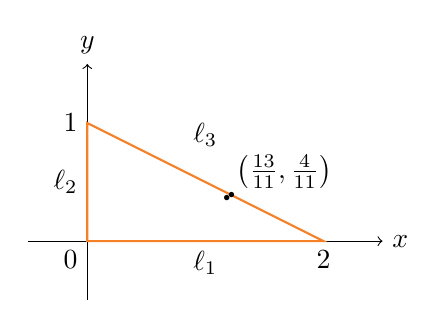
\begin{tikzpicture}[scale=1.5]
          \draw[->] (-0.5,0) -- (2.5,0) node[right] {\(x\)};
          \draw[->] (0,-0.5) -- (0,1.5) node[above] {\(y\)};
          \draw[color=horange, thick] (0,0) -- (2,0) -- (0,1) -- cycle;
          \node[below left] at (0,0) {\(0\)};
          \node[below] at (2,0) {\(2\)};
          \node[left] at (0,1) {\(1\)};
          \node[below] at (1,0) {\(\ell_{1}\)};
          \node[left] at (0,0.5) {\(\ell_{2}\)};
          \node at (1,0.9) {\(\ell_{3}\)};
          \node[scale=0.5] at (13/11, 4/11) {\(\bullet\)};
          \node[above right] at (13/11, 4/11) {\(\left(\tfrac{13}{11}, \tfrac{4}{11}\right)\)};
          \node[scale=0.5] at (11/9, 7/18) {\(\bullet\)};
      \end{tikzpicture}
    \end{multicols}
    With these values, we can see that the absolute maximum is \(\boxed{-0.083}\) at the point \(\boxed{\left(0, \frac{1}{6}\right)}\) and the absolute minimum is \(\boxed{-1.363}\) at the point \(\boxed{\left(\frac{13}{11}, \frac{4}{11}\right)}\).

    }
    \item (1 point each) Convert each as indicated; leave each answer as exact:
    \begin{enumerate}
        \item Convert the rectangular point \((-5,1)\) to polar coordinates.
        \item Convert the cylindrical point \((5, \frac{7\pi}{6}, 2)\) to rectangular.
        \item Convert the rectangular point \((-2,4,-1)\) to spherical.
        \item Convert the spherical point \((4, \frac{11\pi}{6}, \frac{3\pi}{4})\) to cylindrical.
    \end{enumerate}
    \item (3 points) Determine the value of each given integral. You need to do the work here by hand, but of course can check any answers with technology.
    \begin{enumerate}
      \item \(\displaystyle\iint_{D}(x^{2} + 6xy) \, dA\) where \(D\) is the triangle with vertices \((0,0)\), \((4,0)\), and \((0,12)\).
      \item \(\displaystyle\int_{0}^{2}\int_{x^{2}}^{4} 4x^{3}\cos(y^{3}) \,dy\,dx\)
      \item \(\displaystyle\int_{-3}^{3}\int_{0}^{\mysqrt{9-x^{2}}} \sin(5x^{2} + 5y^{2}) \,dy\,dx\)
      \item \(\displaystyle\int_{0}^{1}\int_{0}^{\mysqrt{1-x}}\int_{0}^{\mysqrt{1-x^{2}-y^{2}}} \mysqrt{x^{2} + y^{2} + z^{2}} \,dz\,dy\,dx\)
    \end{enumerate}
    \item (3 points) Find the volume of the solid described by \(x^{2} + y^{2} \leq 1, \quad x \geq 0, \quad 0 \leq z \leq 4 - y\).
    \item (3 points) Find the average value of the function \(f(x,y) = x\sin(y)\) over the region enclosed by \(y = 0\), \(y = x^{2}\), and \(x = 1\).
    \item (3 points) Find the volume of the solid that lives within both the cylinder \(x^{2} + y^{2} = 1\) and sphere \(x^{2} + y^{2} + z^{2} = 9\). \\
    \sol{
        Use cylindrical coordinates. 
    }
\end{enumerate}


\end{document}
